% ****************************************************************************************************
\chapter{Introduction}\label{ch:intro}
% ****************************************************************************************************

\section{Motivation}\label{ch:intro:mo}

\begin{itemize}
	\item "Understand the key elements and mechanisms in a specific business domain, as well as their relationships (Osterwalder \& Pigneur, 2002)", \citep[p. 303]{Pateli2004}
	\item "Focuses on describing the elements and relationships that outline how a company creates and markets value", \citep[p. 7]{Osterwalder2005}
	\item "Modern business models are increasingly complex, particularly those with strong ICT and ebusiness components. The relationship between the different elements of a business model and the decisive success factors are not always immediately observable. Therefore the process of modelling social systems and, in this case, business models help identify and understand the relevant elements in a specific domain and the relationships among them [Morecroft 1994; Ushold and King 1995]. In addition, the visual representation of a business model usually enhances understanding.", \citep[p. 14]{Osterwalder2005}
	\item "As simple as this framework may seem, its power lies in the complex interdependencies of its parts. Major changes to any of these four elements affect the others and the whole. Successful businesses devise a more or less stable system in which these elements bond to one another in consistent and complementary ways.", \citep[p. 53]{Johnson2008}
	\item "A useful way to represent business models is by means of a causal loop diagram, where choices and consequences are linked by arrows based on causality theories" \citep[p. 198]{Casadesus-Masanell2010}
\end{itemize}


\section{Research Objectives}\label{ch:intro:ro}

Classify PaaS providers' business models and its main components. Reveal crucial interdependencies within PaaS business models elements with regards to the platform adoption, using the concept of system dynamics.

\begin{MRQ}\label{mrq}
How to design Platform as a Service business models in order to achieve a high adoption rate?
\end{MRQ}

\begin{SRQ}\label{srq1}
How can business models of Platform as a Service providers' be classified?
\end{SRQ}

\begin{SRQ}\label{srq2}
How are the Platform as a Service business model elements -- especially in regards to the platform adoption -- interrelated?
\end{SRQ}

\thref{mrq}\\
\thref{srq1}\\
\thref{srq2}
	
\section{Research Methodology and Structure}\label{ch:intro:met}

Design Science Research:
\begin{itemize}
	\item \citet{March1995}
	\item \citet{Hevner2004}
	\item \citet{Hevner2007}
	\item \citet{Peffers2007}
\end{itemize}

\begin{figure}[htb]
	\centering
	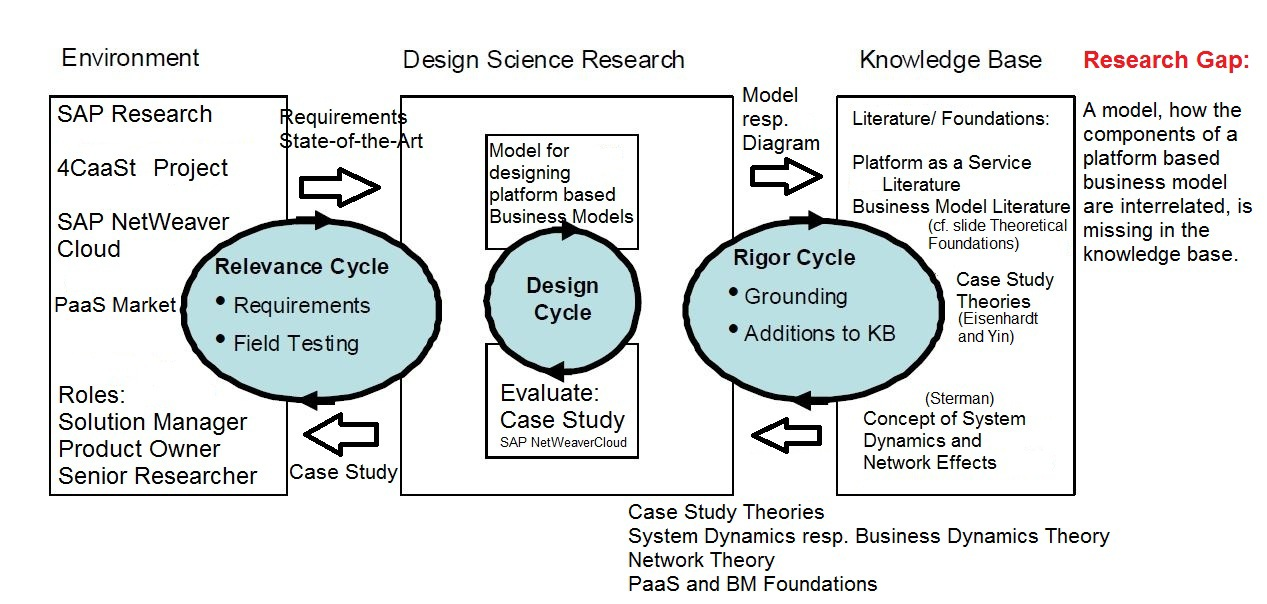
\includegraphics[width=\textwidth]{gfx/researchMethodology}
	\caption[Research Methodology]{Research Methodology adapted from \citet{Hevner2007}}
	\label{fig:rm}
\end{figure}

\begin{figure}[tb]
	\centering
	% ****************************************************************************************************
% Design Science Research
% ****************************************************************************************************

\begin{tikzpicture}[scale=0.75, every node/.style={scale=0.75}, node distance = 4.5cm]

\node[draw,text width=8em,text centered, rectangle,rounded corners,minimum height=4em,thick,rotate=90] (a1) {
	\begin{minipage}{8em}\centering
		Identify\\ Problem\\ \& Motivate\\
		~\\
		\textit{Emerging \ac{PaaS} Market\\~\\Importance of strategy and ecosystems for platform-based business models.}
		~\\~\\~\\~\\~\\~\\~\\~\\
		(cf. Chapter \ref{ch:intro:mo})
		\\~
	\end{minipage}
};

\node[draw,text width=8em,text centered,rectangle,rounded corners,minimum height=4em,thick,rotate=90, right of=a1] (a2) {
\begin{minipage}{8em}\centering
		Define\\ Objectives of\\ a Solution\\
		~\\
		\textit{Classify PaaS providers' business models and its main components. Reveal crucial interdependencies within PaaS business models elements with regards to the platform adoption, using the concept of system dynamics.}
		~\\~\\
		(cf. Chapter \ref{ch:intro:ro})
		\\~
	\end{minipage}
};

\node[draw,text width=8em,text centered,rectangle,rounded corners,minimum height=4em,thick,rotate=90, right of=a2] (a3) {
\begin{minipage}{8em}\centering
		Design \&\\ Development\\
		~\\~\\
		\textit{Elaboration of a classification scheme for \ac{PaaS} business models. Development of a system dynamics model to demonstrate the adoption of platform-based business models.}
		~\\~\\~\\~\\~\\
		(cf. Chapter \ref{ch:sota} and \ref{ch:sd})
	\end{minipage}
};

\node[draw,text width=8em,text centered,rectangle,rounded corners,minimum height=4em,thick,rotate=90, right of=a3,] (a4) {
\begin{minipage}{8em}\centering
		Demonstration\\
		~\\~\\~\\
		\textit{By classifying several \ac{PaaS} business models the usability of the classification scheme is demonstrated. Through modeling actual\ldots}
		~\\~\\~\\~\\~\\~\\~\\
		(cf. Chapter \ref{ch:e})
		\\~
	\end{minipage}
};

\node[draw,text width=8em,text centered,rectangle,rounded corners,minimum height=4em,thick,rotate=90, right of=a4] (a5) {
\begin{minipage}{8em}\centering
		Evaluation\\
		~\\~\\~\\
		\textit{The developed classification scheme as well as the system dynamics model is evaluated in an interactive approach trough a focus group and expert interviews.}
		~\\~\\~\\~\\~\\~\\
		(cf. Chapter \ref{ch:e})
		\\~
	\end{minipage}
};

\node[draw,text width=8em,text centered,rectangle,rounded corners,minimum height=4em,thick,rotate=90, right of=a5] (a6) {
\begin{minipage}{8em}\centering
		Communication\\
		~\\~\\~\\
		\textit{As of writing this paper at hand, it is planned to write and submit a conference paper for the 47th \ac{HICSS}.}
		~\\~\\~\\~\\~\\~\\
	\end{minipage}
};

\node[draw,text width=5em,text centered,circle,rounded corners,minimum height=4em,thick,rotate=90, below of=a1,node distance=8cm] (e) {Problem-Centered Initiation};

\node[rotate=90, above left=3.51em and 1cm of a6] (ao6) {};
\node[rotate=90, above left=3.51em and 1cm of a5] (ao5) {};
\node[rotate=90, above left=3.51em and 1cm of a3] (ao3) {};
\node[rotate=90, above left=3.51em and 1cm of a2] (ao2) {};

%(a4.east)+(-1,0)

\path 
	(a1.70) edge [->,thick,>=stealth'] node [rotate=180,above left=0.2cm and 0cm of a1]{Inference} (a2.110)
	(a2.70) edge [->,thick,>=stealth'] node [rotate=180,above left=0.26cm and 0cm of a2]{Theory} (a3.110)
	(a3.70) edge [->,thick,>=stealth'] node [rotate=180,above left=0.26cm and 0cm of a3]{How to Knowledge} (a4.110)
	(a4.70) edge [->,thick,>=stealth'] node [rotate=180,above left=0.26cm and 0cm of a4]{Metrics, Analysis Knowledge} (a5.110)
	(a5.70) edge [->,thick,>=stealth'] node [rotate=180,above left=0.26cm and 0cm of a5]{Disciplinary Knowledge} (a6.110)
	(e.north) edge [->,thick,>=stealth'] (a1.south)
	
	(a6.north) edge [-,thick,>=stealth'] (ao6.south)
	(a5.north) edge [-,thick,>=stealth'] (ao5.south)
	(a3.north) edge [-,thick,>=stealth'] (ao3.south)
	(ao6.south) edge [-,thick,>=stealth'] node [rotate=90, above left=3.18em and 0.1cm of a4]{Process Iteration} (ao2.south)
	(ao3.south) edge [->,thick,>=stealth'] (a3.north)
	(ao2.south) edge [->,thick,>=stealth'] (a2.north);

\end{tikzpicture}


	\caption[Design Science Research Methodology -- Process Model]{Design Science Research Methodology -- Process Model, adapted from \citet{Peffers2007}}
	\label{fig:dsrm}
\end{figure}

